\subsubsection{SỰ PHÁT TRIỂN MÔ HÌNH NGUYÊN TỬ}
\begin{tomtat}
	\begin{minipage}[htp!]{0.5\textwidth}
		Từ thời cổ Hy Lạp,nhà triết học Democritous (Đê-mô-crít) (Hình \ref{fig:Democritus})
		Mọi thứ trên thế giới đều được tạo ra từ các hạt nhỏ không thể chia nhỏ được nữa được gọi là \textbf{“nguyên tử”}, có nghĩa là \textbf{“không thể thay đổi được”}
	\end{minipage}
	\begin{minipage}[htp!]{0.5\textwidth}
		\begin{center}
			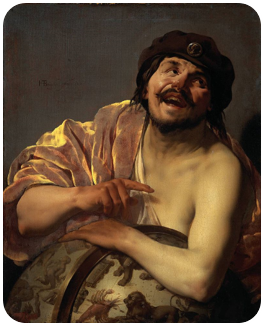
\includegraphics[width=3cm]{Images/anhhoahoc10/DEMOCRITUS.png}
			\captionof{figure}{Democritus (460 - 370,Hy Lạp)\label{fig:Democritus} }
		\end{center}
	\end{minipage}
	
	\begin{center}
		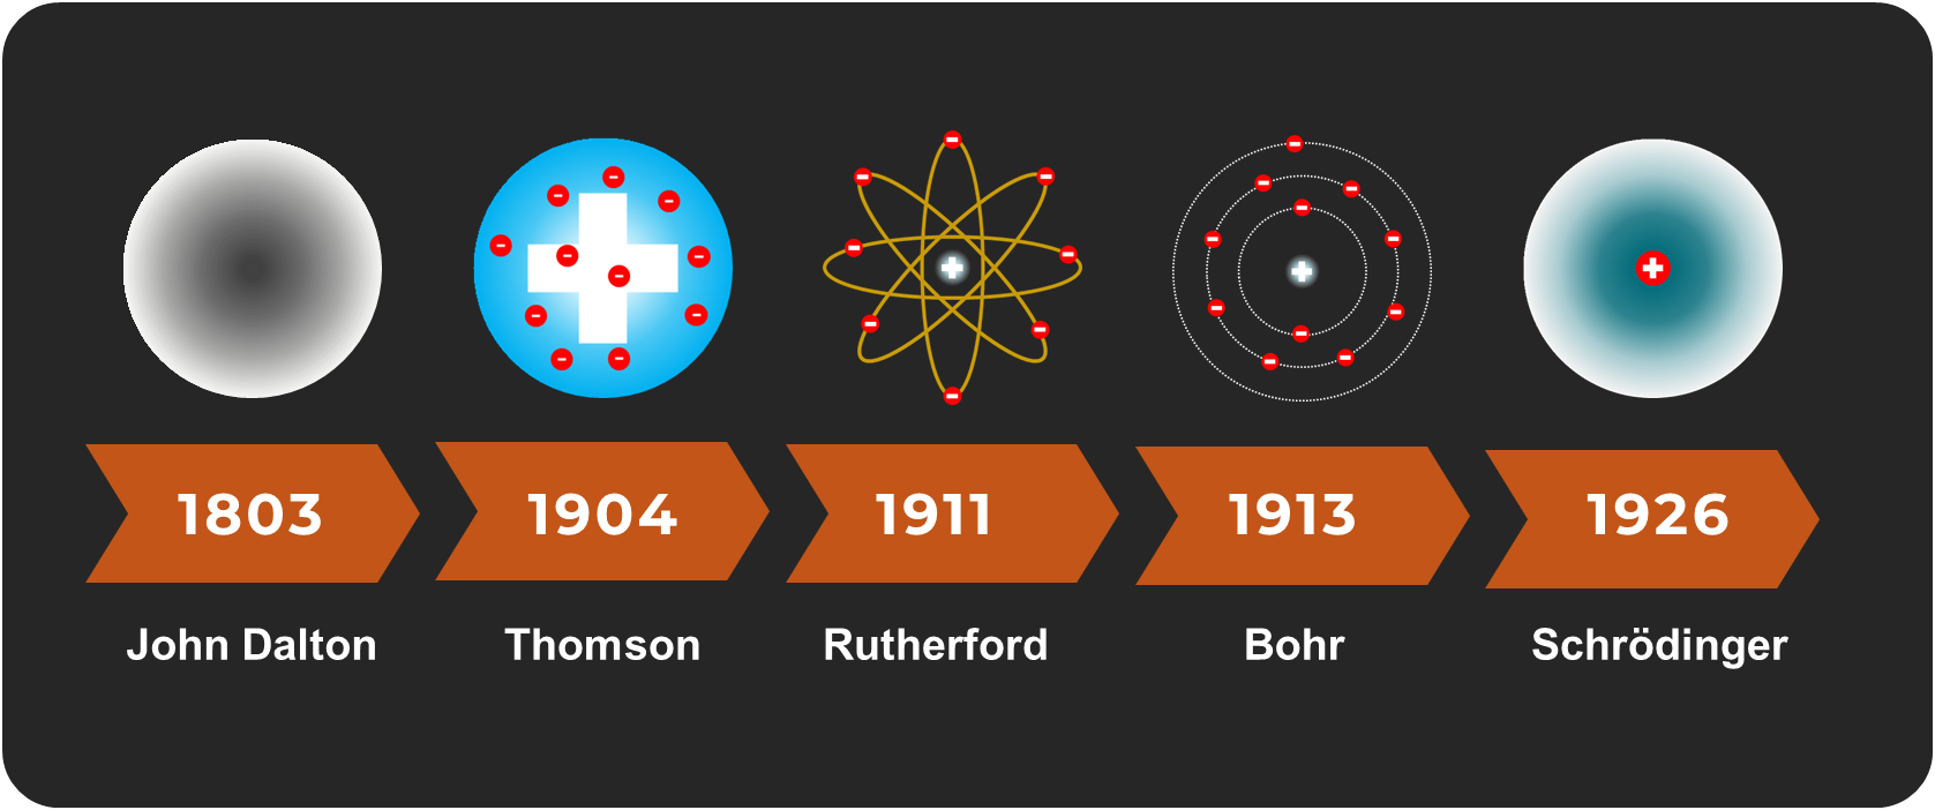
\includegraphics[width=12cm]{Images/anhhoahoc10/historyatom.png}
		\captionof{figure}{Lịch sử phát triển mô hình nguyên tử \label{fig:Historyatom} }
	\end{center}
\end{tomtat}
\subsubsection{Thành phần và cấu trúc của nguyên tử}
\Noibat[][][\faArrowCircleOLeft]{Thành phần}
\vspace{0.5cm}
\begin{tomtat}
	Nguyên tử gồm hạt nhân chứa proton, neutron và vỏ nguyên tử chứa electron.
	\begin{center}
		\includegraphics[width=9cm]{Images/anhhoahoc10/mohinhnguyentu.png}
		\captionof{figure}{Mô hình nguyên tử}
	\end{center}
\end{tomtat}
\subsubsection{Sự tìm ra electron}
\Noibat[][][\faArrowCircleOLeft]{Thí nghiệm khám phá tia âm cực của Thomson}\\
Năm 1897, J. J. Thomson (Tôm-xơn, người Anh) thực hiện thí nghiệm phóng điện qua không khí loãng đã phát hiện ra chùm tia phát ra từ cực âm.(xem hình \ref{fig:hinh3} ) và link video bằng mã QR ở bên dưới.\\ 
\hinhphai{\begin{center}
		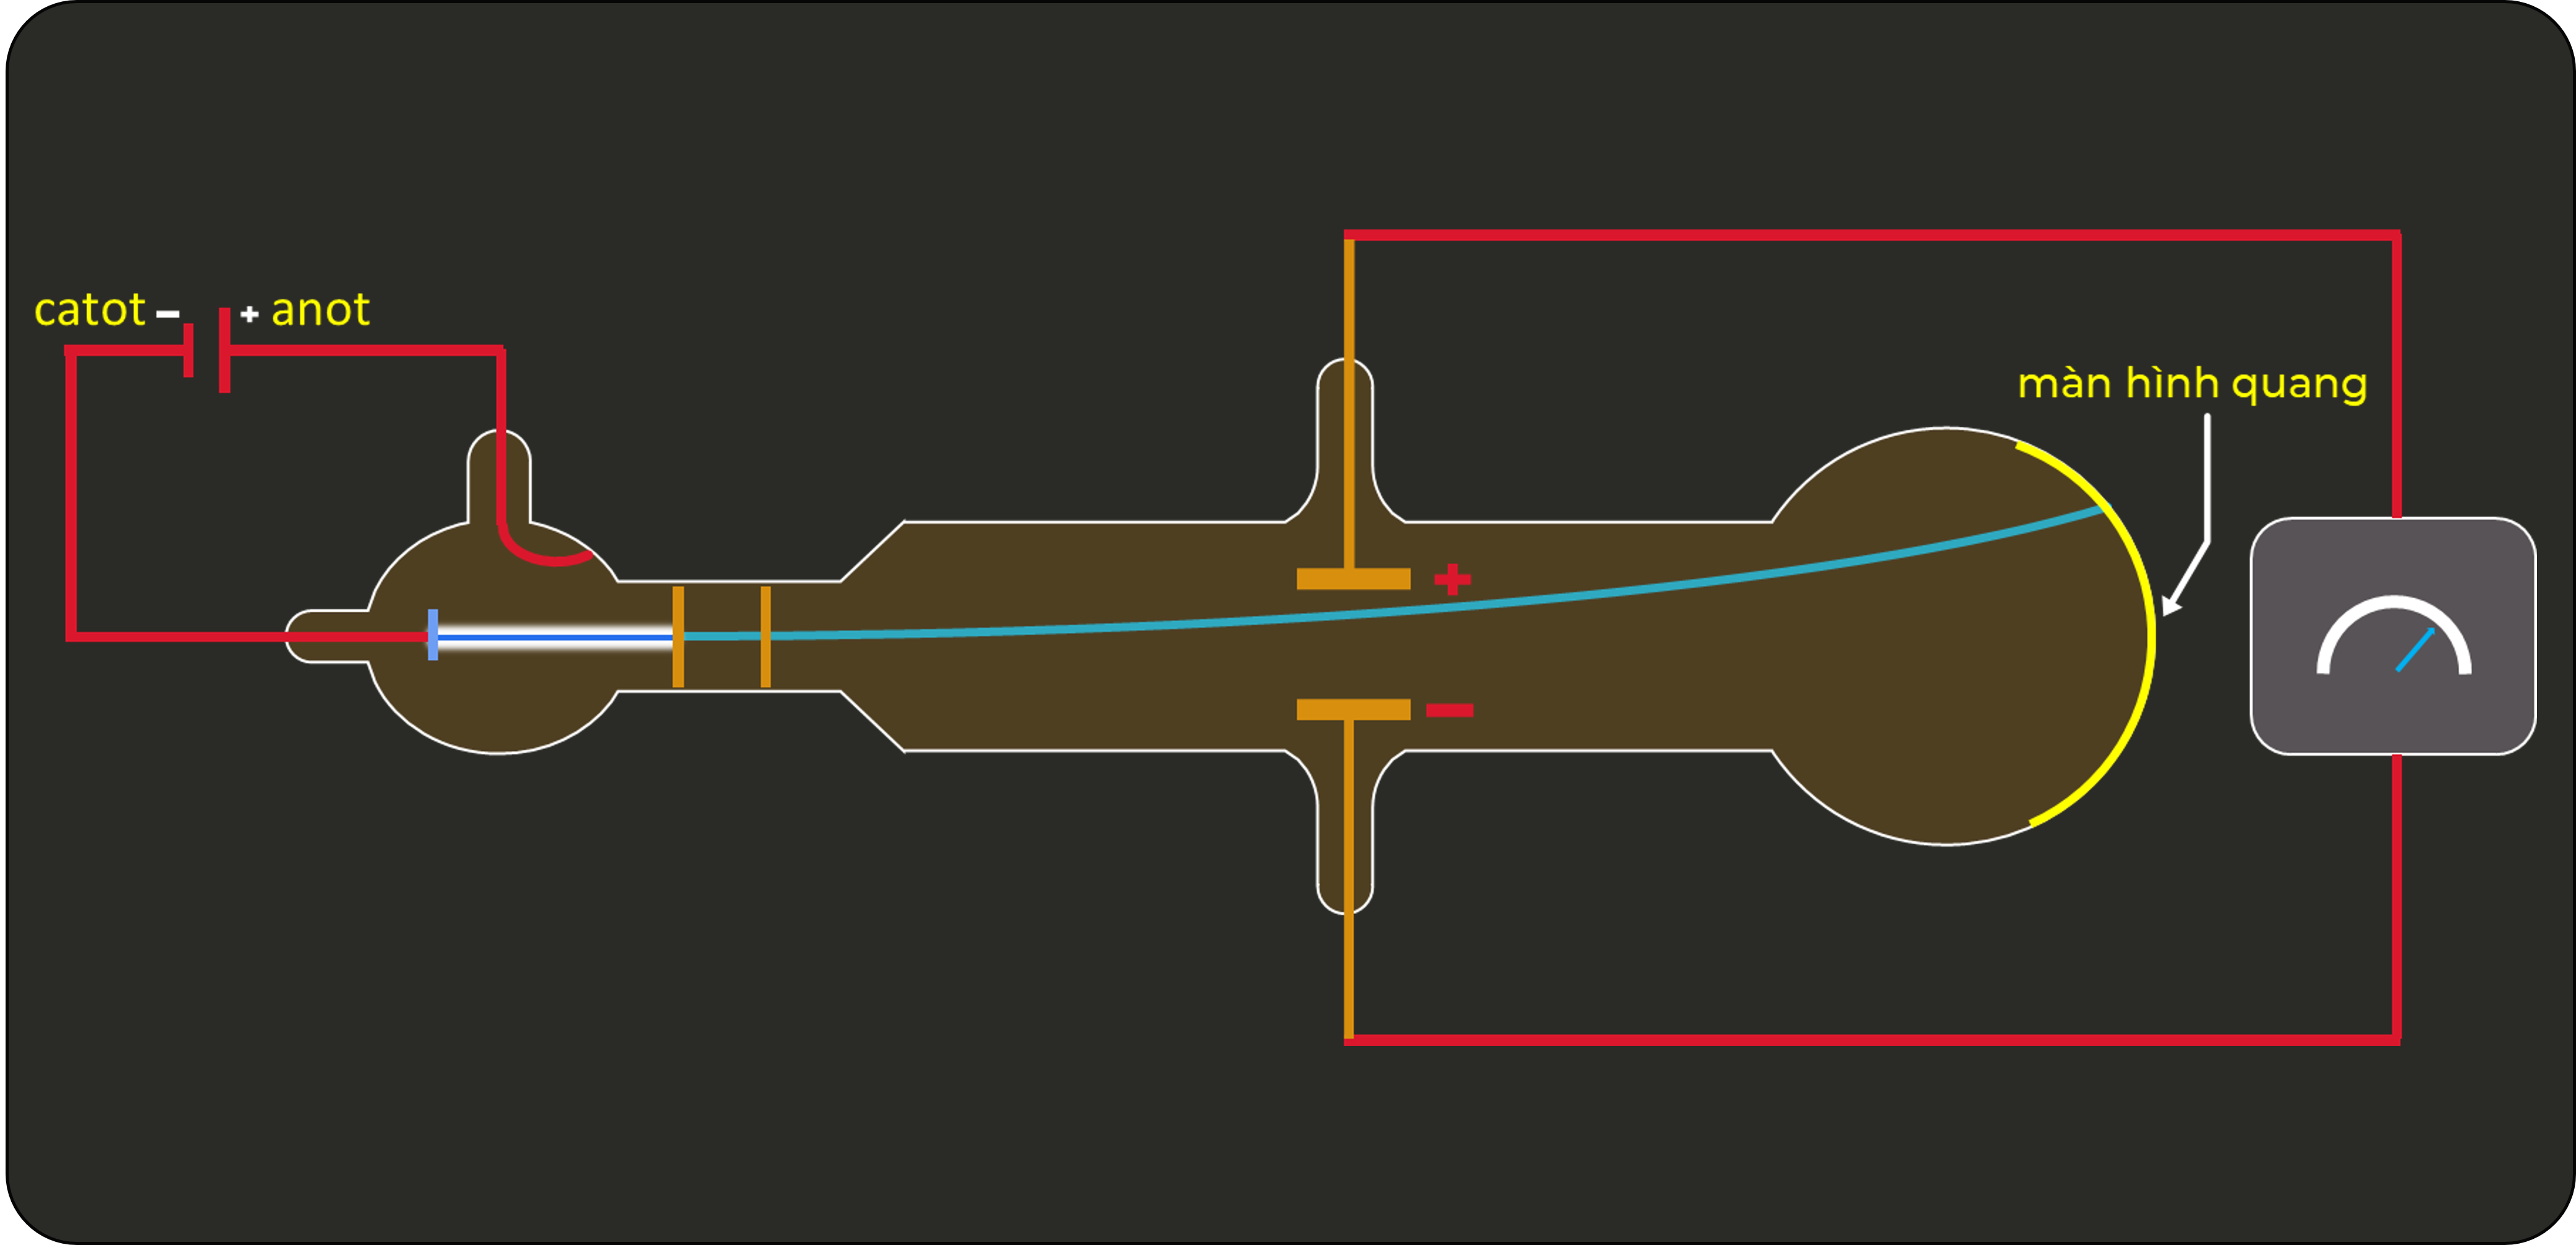
\includegraphics[width=9cm]{Images/anhhoahoc10/TNTHOMSON.png}\\
		\captionof{figure}{Thí nghiệm của Thomson}
		\label{fig:hinh3}
\end{center}}{\begin{tikzpicture}
		\path (0,0)  node (QRCODE) {\maqr[\maunhan][3]{https://youtu.be/y2uswXtC5O8}}
		(QRCODE.south) node[anchor=north]{(\fmmfamily Các bạn  dùng ~\rotatebox{-15}{\faMobile}~quét mã QR để xem video TN nhé!)}
		;
\end{tikzpicture}}

\begin{hoivadap}
	\begin{cauhoi}
		Vai trò của lớp bột huỳnh quang trong thí nghiệm ở hình \ref{fig:hinh3}
	\end{cauhoi}
	\loigiai{\taodongke{3}}
\end{hoivadap}

\begin{hoivadap}
	\begin{cauhoi}
		Quan sát Hình \ref{fig:hinh3} và video , giải thích vì sao tia âm cực bị hút về cực dương của trường điện.
	\end{cauhoi}
	\loigiai{\taodongke{3}}
\end{hoivadap}
%
\begin{hoivadap}
	\begin{cauhoi}
		Nếu đặt một chong chóng nhẹ trên đường đi của tia âm cực thì chong chóng sẽ quay. Từ hiện tượng đó, hãy nêu kết luận về tính chất của tia âm cực.
	\end{cauhoi}
	\loigiai{\taodongke{3}}
\end{hoivadap}

\begin{Bancobiet}
	Mô hình Thomson còn gọi là mô hình \lq\lq bánh pudding mận".Theo Thomson:
	\begin{enumerate}
		\item Nguyên tử là quả cầu mang điện tích dương, bên trong chứa các êlectron.
		\item Nguyên tử trung hòa về điện.
	\end{enumerate}
\end{Bancobiet}
%
%
\subsubsection{Sự khám phá hạt nhân nguyên tử}
\Noibat[][][\faArrowCircleOLeft]{Tìm hiểu thí nghiệm của Rutherford}\\
Năm 1911, E. Rutherford (Ro-dơ-pho, người Niu Di-lân) thực hiện thí nghiệm bắn phá lá vàng rất mỏng bằng chùm hạt $ \alpha $ \footnote{Hạt $\alpha$ : hạt nhân helium, mang điện tích dương.} (xem hình \ref{fig:hinh4})
\begin{center}
	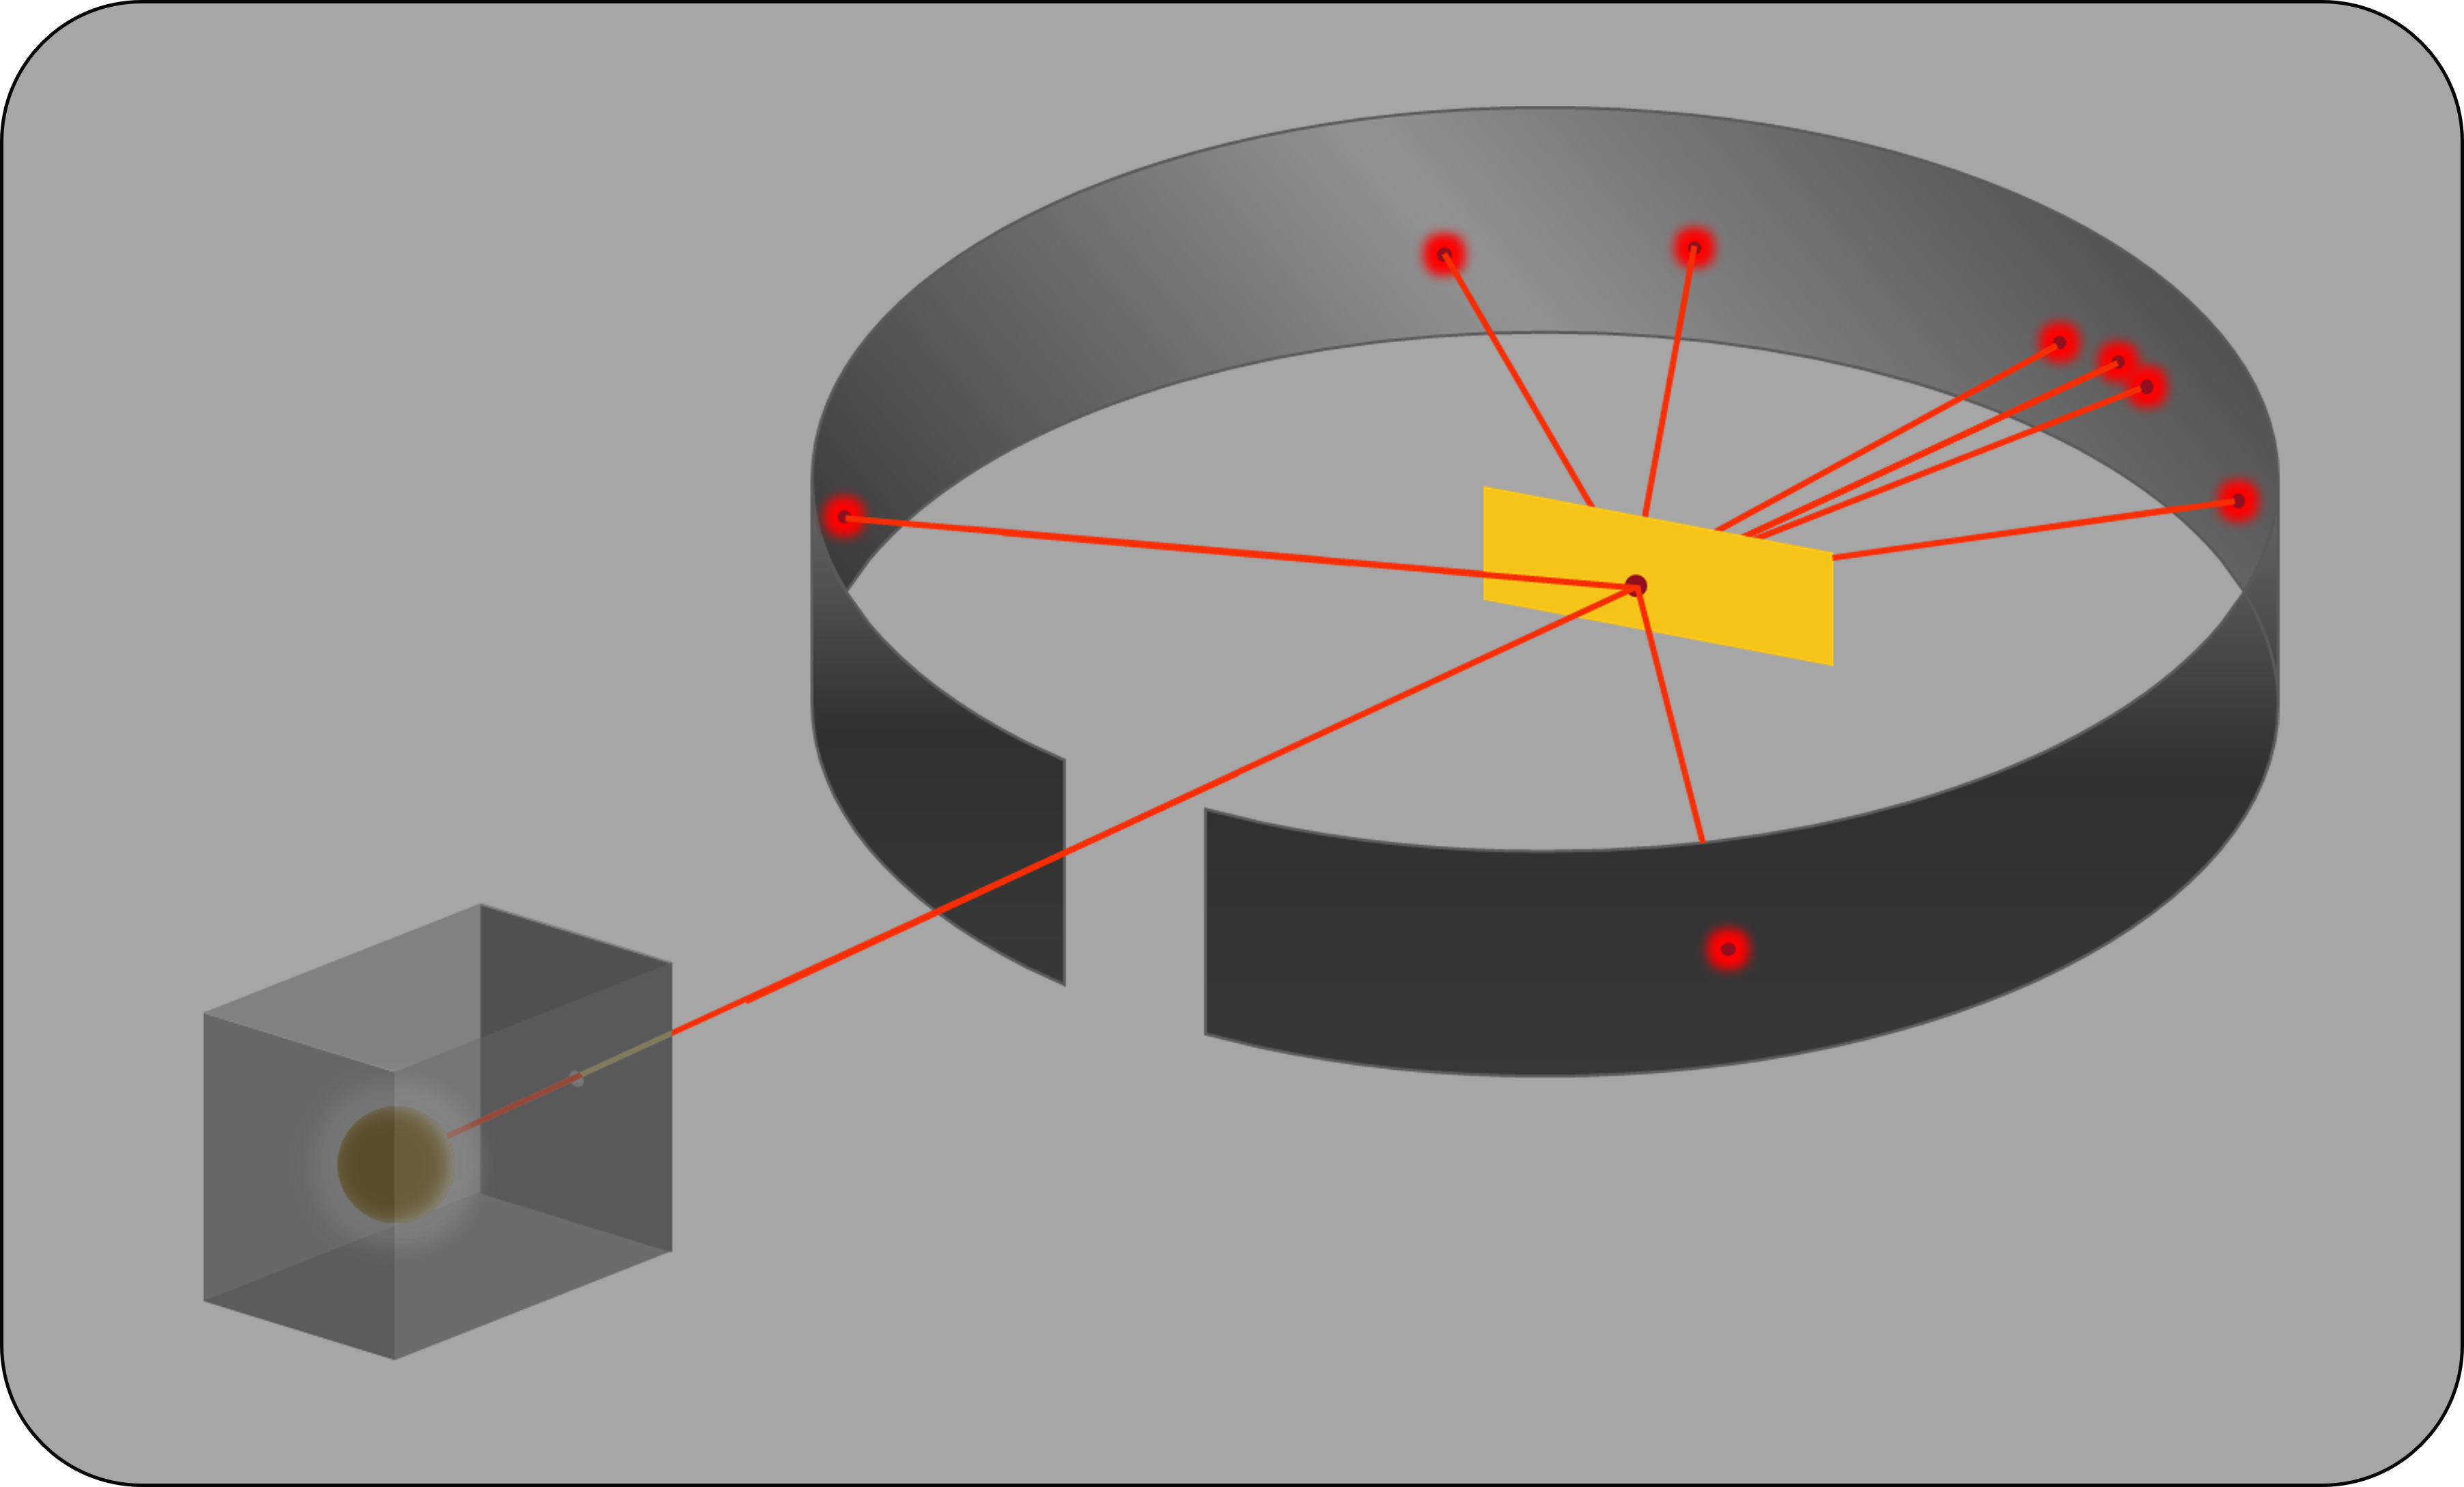
\includegraphics[width=9cm]{Images/anhhoahoc10/TNRUTHERFORT.png}\\
	\captionof{figure}{Thí nghiệm của Rutherford}
	\label{fig:hinh4}
\end{center}

\begin{center}
	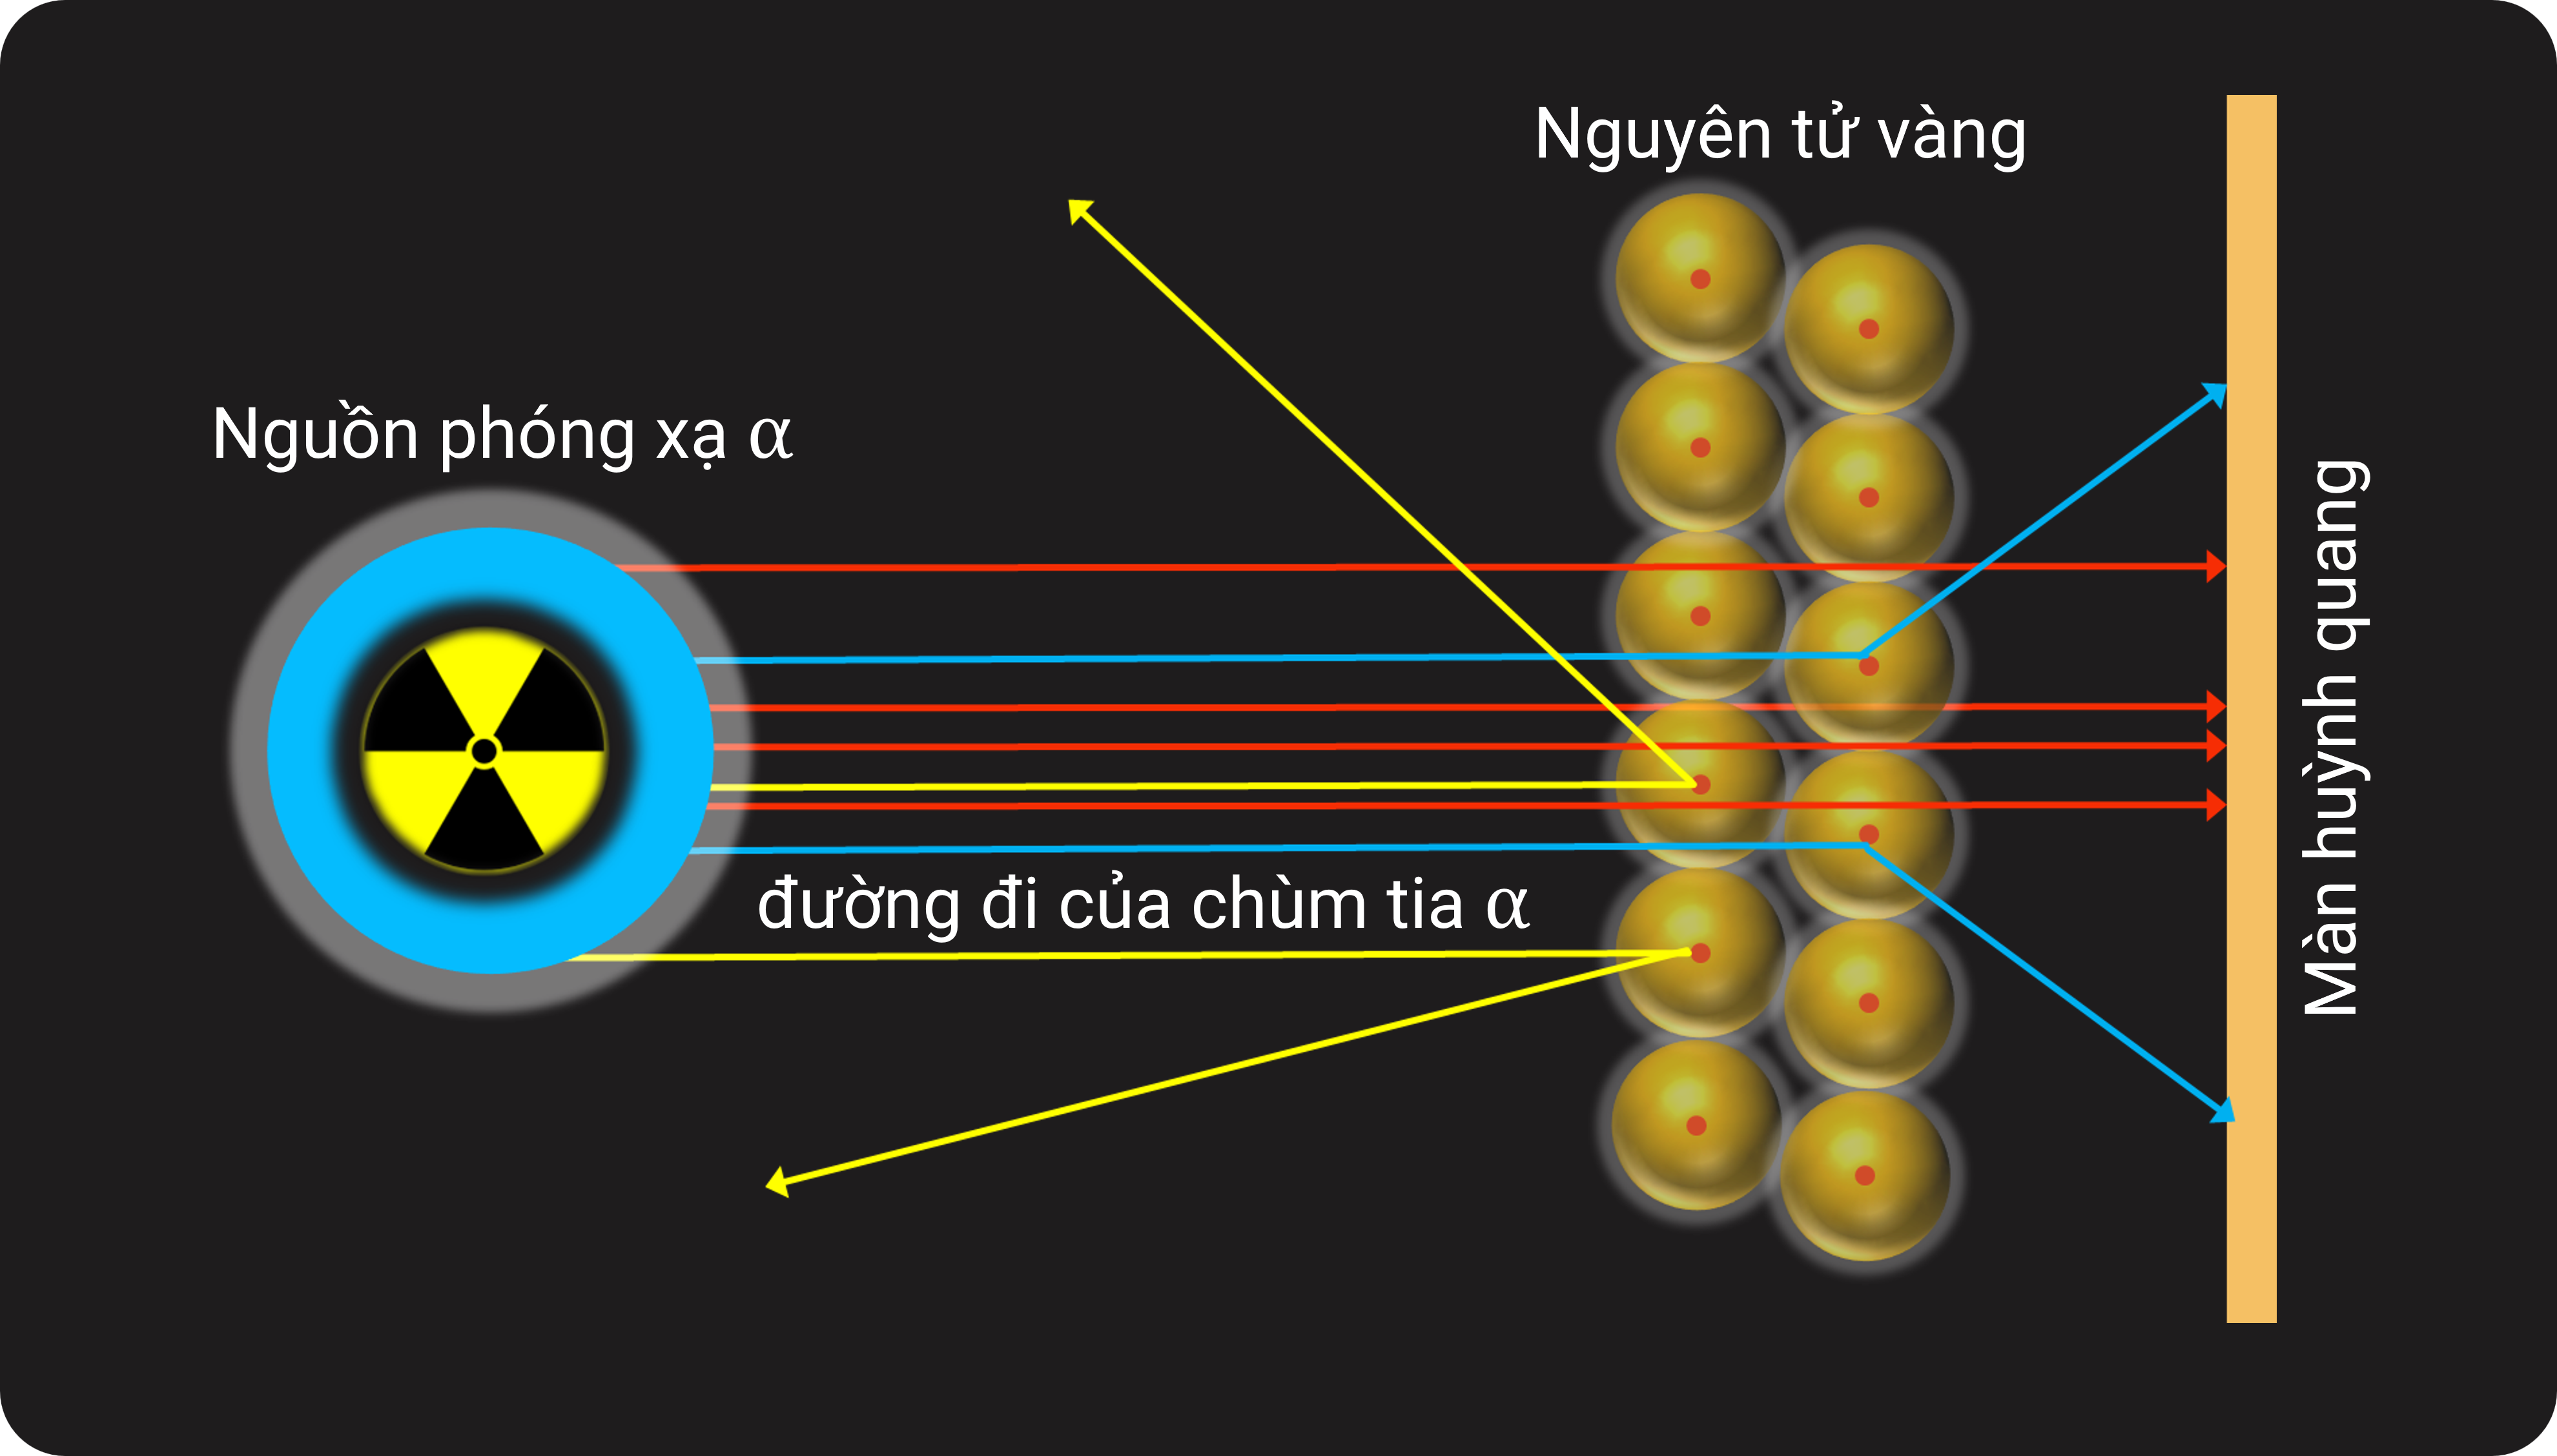
\includegraphics[width=9cm]{Images/anhhoahoc10/KQTN.png}\\
	\captionof{figure}{Kết quả thí nghiệm của Rutherford}
	\label{fig:hinh5}
\end{center}
%
\begin{hoivadap}
	\begin{cauhoi}
		Quan sát hình \ref{fig:hinh4}, cho biết các hạt $\alpha$ có đường đi như thế nào. Dựa vào Hình \ref{fig:hinh5} , giải thich kết quả thí nghiệm thu được.
	\end{cauhoi}
	\loigiai{\taodongke{5}}
\end{hoivadap}
%\vspace*{6pt}
\begin{tomtat}
	{\bfseries{Kết luận}}
	\begin{itemize}
		\item Nguyên tử có cấu tạo rỗng, gồm hạt nhân ở trung tâm và lớp vỏ là các electron chuyển động xung quanh hạt nhân.
		\item Nguyên tử trung hoà về điện: số đơn vị điện tích dương của hạt nhân bằng số đơn vị điện tích âm của các electron trong nguyên tử.
	\end{itemize}
\end{tomtat}
\subsubsection{Cấu tạo hạt nhân nguyên tử}
\begin{center}
	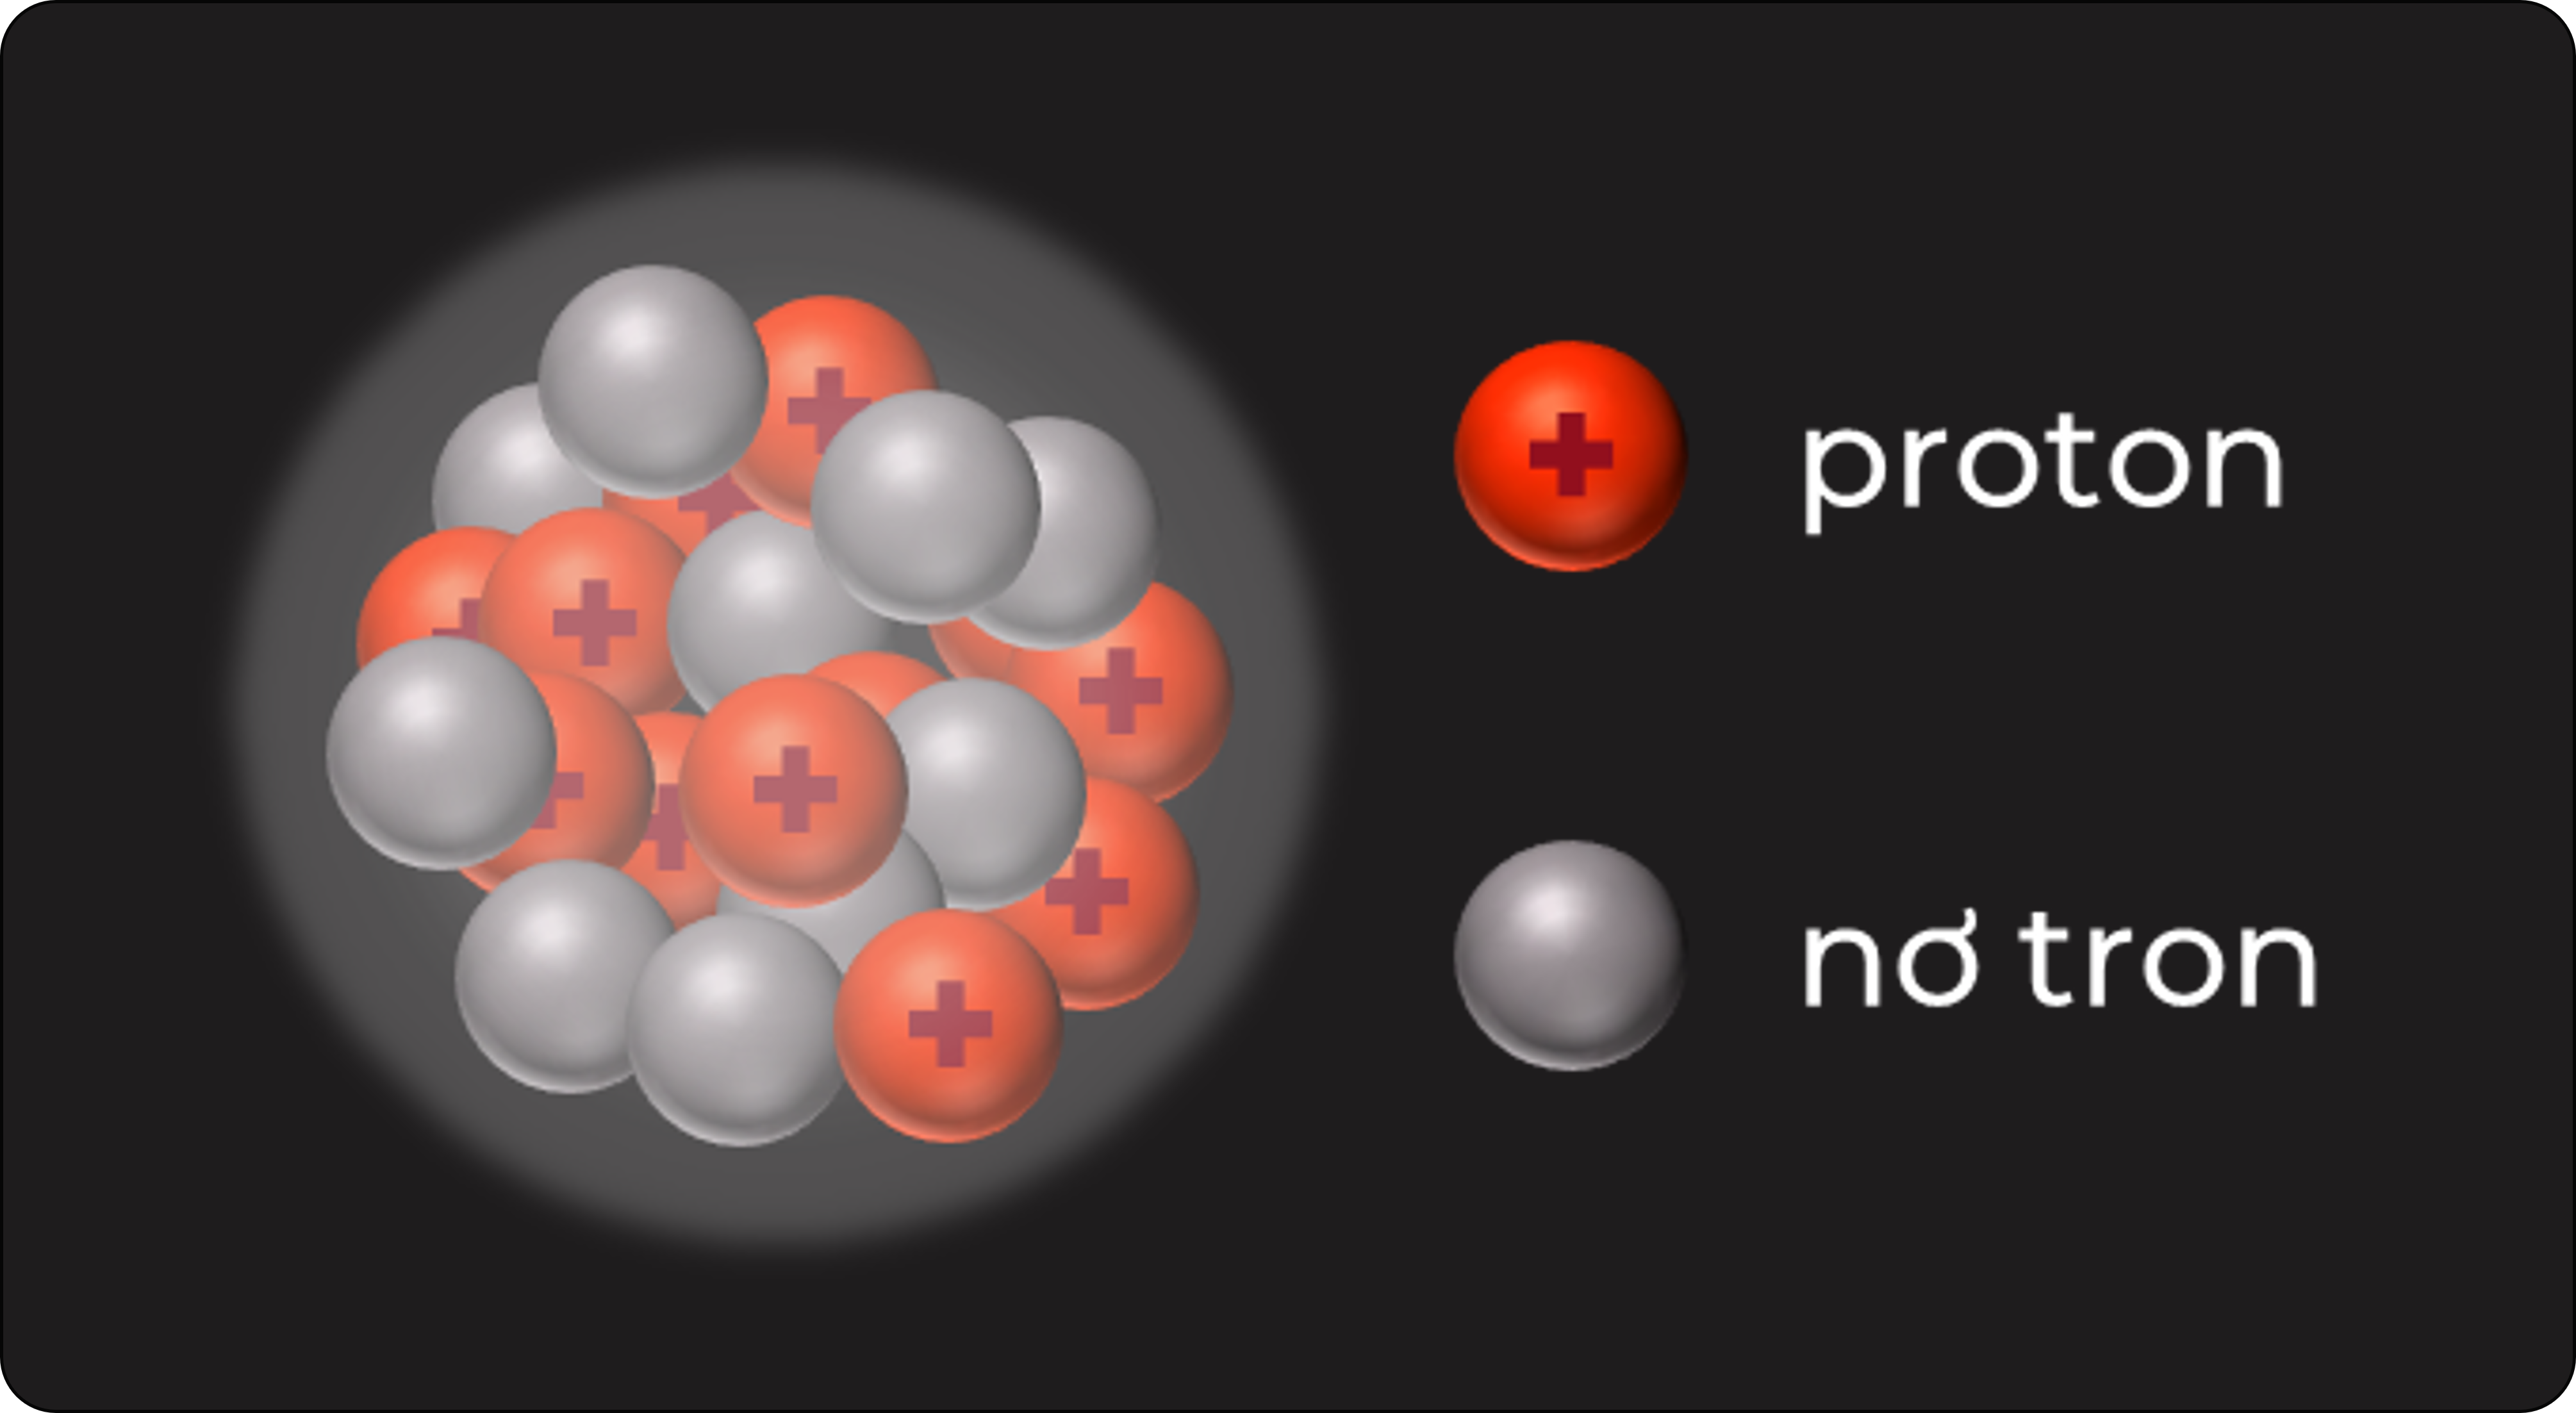
\includegraphics[width=9cm]{Images/anhhoahoc10/CAUTAOHATNHAN.png}\\
	\captionof{figure}{Thành phần của hạt nhân}
	\label{fig:hinh6}
\end{center}
\begin{hoivadap}
	\begin{cauhoi}
		Quan sát hình \ref{fig:hinh6} và kết hợp SGK , các bạn hãy nêu thành phần của hạt nhân
	\end{cauhoi}
\end{hoivadap}
\begin{ghinho}
	Proton, neutron và electron là các hạt cấu tạo nên nguyên tử.
\end{ghinho}
\begin{tongket}{Tổng kết}
	Thành phần cấu tạo của nguyên tử gồm:
	\begin{itemize}
		\item  Hạt nhân (nucleus): ở tâm của nguyên tử, chứa các proton mang điện tích dương và các neutron không mang điện.
		\item Vỏ nguyên tử: chứa các electron mang điện tích âm, chuyển động rất nhanh xung quanh hạt nhân.
		\item Trong nguyên tử, số proton bằng số electron nên nguyên tử trung hoà điện.
		\item Khối lượng của electron rất nhỏ, không đáng kể so với khối lượng của proton hay neutron nên khối lượng của nguyên tử tập trung hầu hết ở hạt nhân.
	\end{itemize}
\end{tongket}
%
%
\begin{longtable}{|c|c|c|c|c|c|}
	\caption{\indam[\maunhan]{Khối lượng, điện tích của các loại hạt cấu tạo nên nguyên tử}}
	\label{tab:ktntklnt}\\
	\hline
	\rowcolor{\mauphu!25} \indam[\mauphu]{Hạt} & \indam[\mauphu]{Kí hiệu} & $\begin{array}{c}\text {\indam[\mauphu]{Khối lượng} } \\
		\text {\indam[\mauphu]{(kg)}  }\end{array}$ & \indam[\mauphu]{Khối lượng (amu)} & $\begin{array}{c}\text { \indam[\mauphu]{Điện tích} } \\
		\text { \indam[\mauphu]{(C)} }\end{array}$ & $\begin{array}{l}\text { \indam[\mauphu]{Điện tích} } \\
		\text { \indam[\mauphu]{tương đối} }\end{array}$ \\
	\hline\endhead
	\rowcolor{\mycolor!15} Proton & $p$ & $1,672 \cdot 10^{-27}$ & $\approx 1$ & $1,602 \cdot 10^{-19}$ & +1 \\
	\hline
	\rowcolor{\mycolor!15} Neutron & $\mathrm{n}$ & $1,675 \cdot 10^{-27}$ & $\approx 1$ & 0 & 0 \\
	\hline\rowcolor{\mycolor!15} Electron & e & $9,109 \cdot 10^{-31}$ & $\begin{array}{c}
		~ \\
		\dfrac{1}{1837} \approx 0,00055\\
		~ \\
	\end{array}$ & $-1,602 \cdot 10^{-19}$ & -1 \\
	\hline
\end{longtable}
\subsubsection{Kích thước và khối lượng nguyên tử}
\begin{center}
	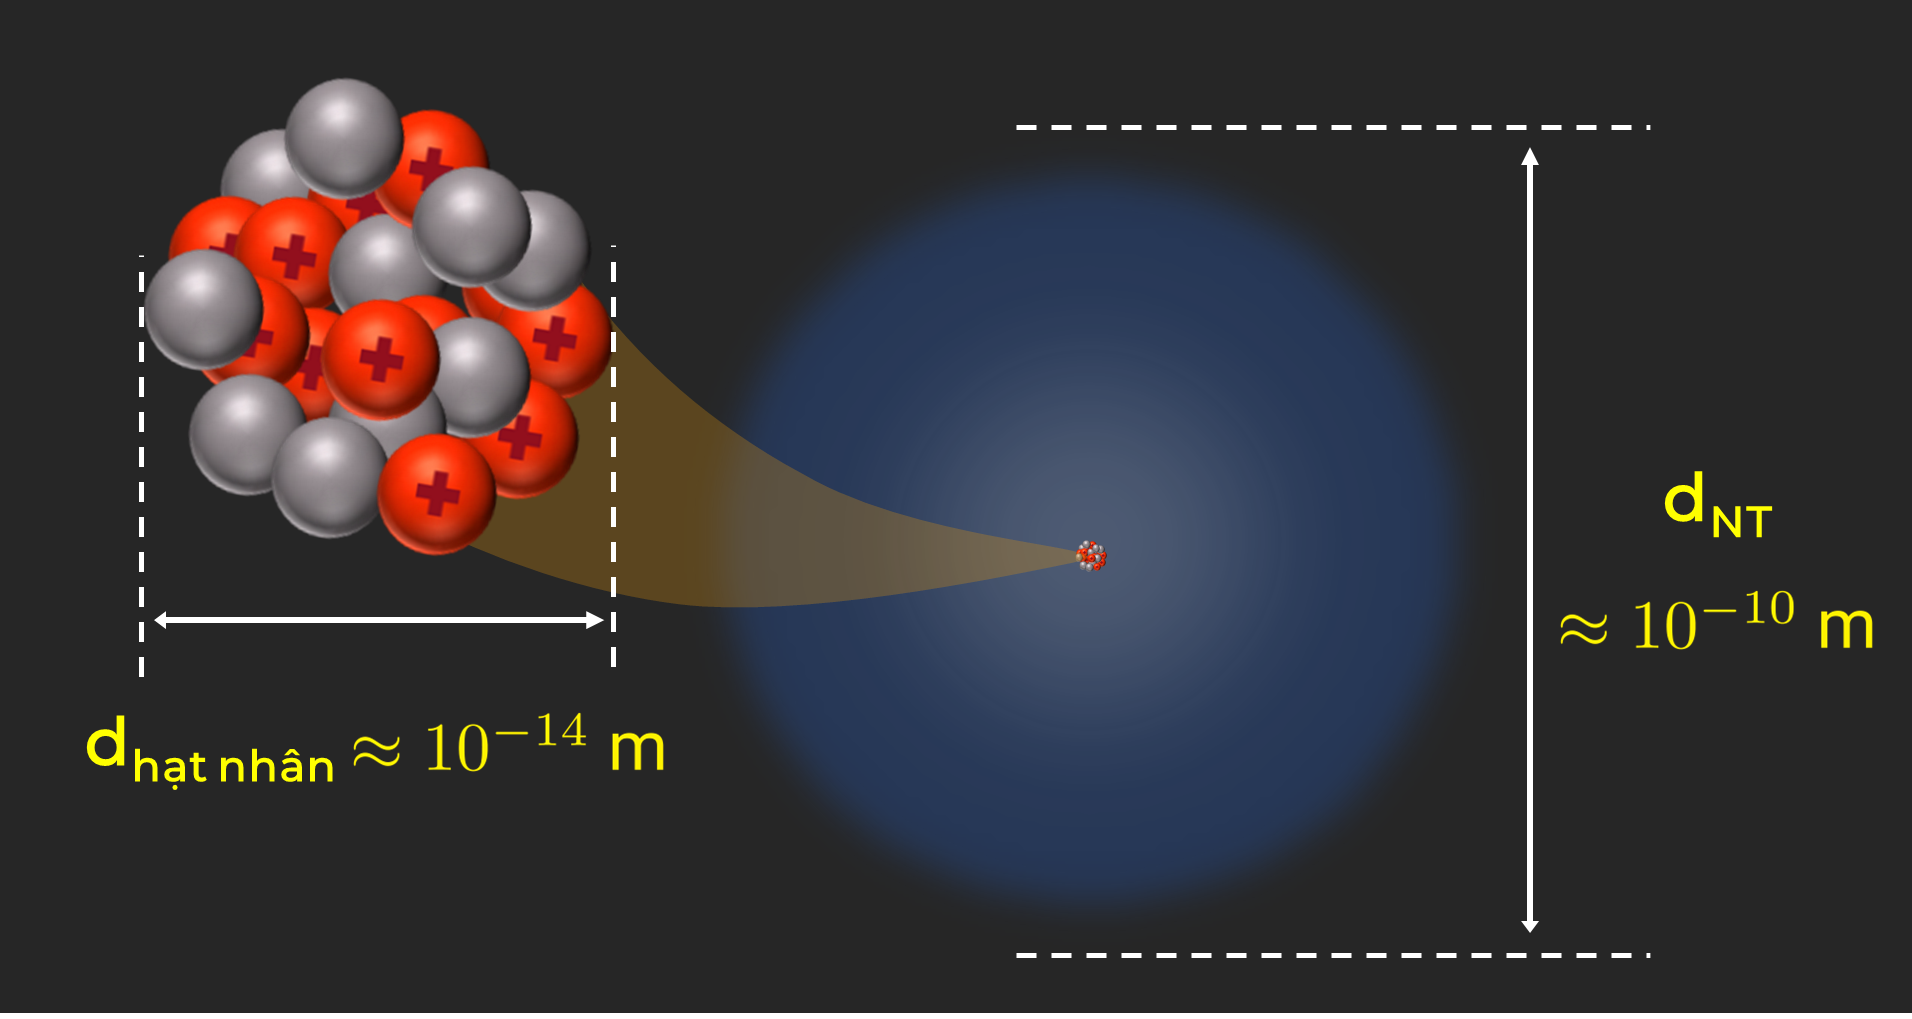
\includegraphics[width=9cm]{Images/anhhoahoc10/ktnt.png}\\
	\captionof{figure}{So sánh kích thước hạt nhân , nguyên tử}
	\label{fig:m-q-hatcoban}
\end{center}
\vspace*{0.25cm}
\begin{note}
	\begin{itemize}
		\item Đơn vị kích thước thường dùng của nguyên tử là Angstron ($ A^0 $) hoặc nano mét (nm)			
		$$1 \mathrm{~nm}=10^{-9}~\mathrm{m} ; 1 A^0=10^{-10}~\mathrm{~m} ; 1 \mathrm{~nm}=10 A^0; 1 A^0=10^{2}~\mathrm{pm}$$
		\begin{center}
			\tcbox[width=5cm,colframe=\maunhan]{$ \dfrac{d_{\text{NT}}}{d_{\text{hạt nhân}}}\approx \dfrac{10^{-10}}{10^{-14}} \approx 10^4~\mathrm{\text{lần}} $}
		\end{center}
		\item Đơn vị của khối lương nguyên tử là amu (atomic mass unit),
		$$
		1 \mathrm{amu}=1,6605 \times 10^{-27} \mathrm{~kg} \text {. }
		$$
		\item Đơn vi của điện tích các hạt cơ bản là $\mathrm{e}_0$ (điện tích nguyên tố),
		$$
		1 \mathrm{e}_0=1,602 \times 10^{-19} \mathrm{C} \text {. }
		$$
	\end{itemize}
\end{note}